\documentclass[11pt]{report}
\usepackage{baththesis}
\usepackage[utf8]{inputenc}
\usepackage{graphicx}
\usepackage{wrapfig}
\usepackage{subcaption}
\usepackage{framed}
\usepackage{caption}
\usepackage{hyperref}
\usepackage{pdfpages}

\title{Mixed Reality Presentations\\Project Proposal, and Literature and Technology Review}
\author{Owen Morgan}
\date{}
\degree{EngD in Digital Entertainment}
\department{Computer Science}
\degreemonthyear{April 2017}
\norestrictions

\begin{document}
\maketitle
\chapter{Introduction}
\begin{figure}[h]
\centering
\begin{subfigure}[b]{0.7\textwidth}  
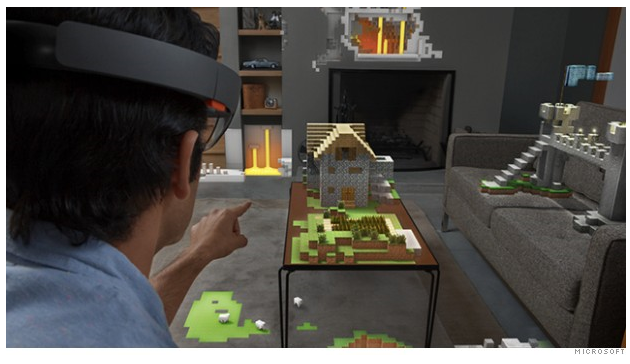
\includegraphics[width=\textwidth]{microsoft-minecraft.png}
\end{subfigure}
\caption{An example rendering of the video game \textit{Minecraft} used in conjunction with Microsoft's MR Hololens.\cite{Hollister2015}}
\end{figure}
\section{Motivation}
Historically, Mixed Reality (MR) applications have focused on a superimposition of virtual elements onto real ones, such as in the Microsoft Hololens device previews (Figure 1-1). However with the rapid research and development into Virtual Reality (VR) technology such as the Vive (Valve/HTC) as well increasing consumer use of VR in smartphones in conjunction with headset adapters, there exists an interesting and unexplored application where MR can be achieved by recording or projecting the real world into a virtual world. Bringing these real world elements into the virtual space is a less explored paradigm compared to the existing MR approaches, and it remains to be studied what benefits, if any, this approach has compared to state of the art. The media of choice for this application will be digital presentations with MR lecturers, viewed in a virtual world. Implementation of such a system could propose benefits in both education engagement and education immersion.
\section{Project Aims}
\begin{figure}
\centering
\begin{subfigure}[b]{0.7\textwidth}  
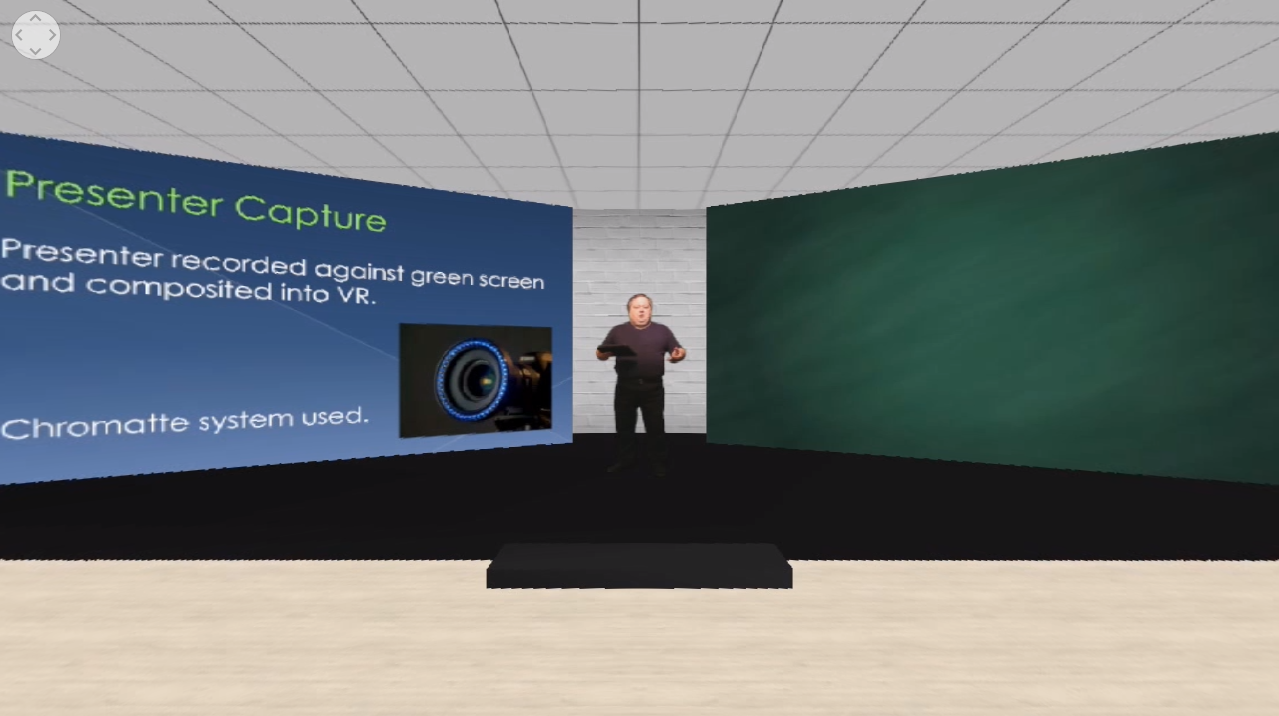
\includegraphics[width=\textwidth]{MRpresentation.png}
\end{subfigure}
\caption{A still image from the 360 playback version of the existing system. The lecturer has placed slides on the left screen and has the ability to draw shapes on the right screen.}
\end{figure}
This project aims to implement a MR system with a green-screen recording of a lecturer embedded into a VR landscape, and to study the efficacy of such a system compared to traditional non-interactive learning mechanisms. Existing work has already been carried out by Ken Cameron, with the program consisting of two components, a capture system and a presentation playback system. The capture system gives the lecturer access to multiple screens with which one can control what's happening on screen, such as drawing on a chalk board. The browser app is written in PHP and Javascript, and syncs up the actions to the presenter to the timing of the video. The actual video itself is shot using green screen capture, and due to the timing based nature of the browser app, the video can be trimmed and edited with the additional content reflecting any video changes. The initial playback system was developed for the Occulus Rift and written in C++, and renders the presenter video as well as anything they created in the browser app. The playback system also includes an export option to 360 video, allowing playback on YouTube's 360 player as well as a number of smartphones. An example of the system is shown in Figure 1-2.\\~\\
The initial objective of this project is to port it from the existing system to the Unity game engine environment. Doing so will pose several advantages, such as platform portability across a variety of devices (e.g. smartphones versus HTC Vive, Occulus Rift) as well as easier maintenance of the game engine playback system. The simple nature of Unity combined with the well organised structure of a game engine will also allow for simple expansion of further research ideas.\\~\\
After this has been completed, additional features for the MR presentation can be considered and implemented. The first element to consider (which would be relatively straightforward to implement in Unity) is a quiz-type system similar to old ``choose your own adventure" style of storytelling. Perhaps in a lecture one might have multiple choice answers to a question, and different parts of the video could play depending on what the answer reply might be. For example, a correct answer given in little time could move the viewer onto a more advance lecture to push the student further, but an incorrect answer could provide the student with a further video on how to better get the correct answer. A further extension on this system would be to allow the lecturer to introduce props into the presentation and allow students in VR to interact with the props, such as in the classic VR application examples of presenting 3D CAD parts. Implementing such as feature in Unity would be relatively straight forward as it would just involve importing and scripting up each prop. More complex props could also be involved, e.g. moving props or props with particle effects. Introduction of props into the lecture can be created from the lecturers web user interface, and perhaps as an eventual end goal, users could create their own props similar to the Steam Workshop present in certain existing VR applications\cite{Education2016}.\\~\\
After the system has been implemented, a study must be performed in order to research whether such an interactive system involving quizzes, props etc., is actually superior to one with a pre-recorded lecture playing simply in VR. To precisely measure this, two lectures on the same topic should be recorded, but one including any interactive elements present in the project. A blind study could be then conducted where participants watch both versions of the project and are quizzed afterwards about what they've learned; the result could be indicative of whether interactive VR learning is worth doing at all or presents any observable improvement in the quality of peoples' learning.\\~\\
A possible project pivot could involve tweaking the system in such a way that a lecturer could present in real time. This objective can be viewed as an extension to the project, and would require a large degree of optimisation in the presentation pipeline. One other pivot in the project may be to reverse the Mixed Reality experience, and present virtual elements in the real world, via the Hololens. This extension may be much more feasible as the pipeline of converting a VR project to an MR project is very straightforward within the Unity engine. What advantages this might bring to the project will be briefly discussed in the literature review. 
\section{Overview}
This report aims to give a detailed look into the state of the art in terms of VR, MR and immersive experiences in education, as well as understanding existing experiences and how the learners are assessed for quality. This report will also examine literature in terms of what makes for an effective immersive experience, not just in education but across the broader VR/AR/MR spectrum, and finally will conclude with a brief technical summary of what technologies and game engines will be used to create the project and a short summary of the proposed time-frame for the project.
\chapter{Literature Review}
\section{Virtual Learning Environments (VLE)}
This section of the literature review will examine the research into and effectiveness on learning of Virtual Learning Environments (VLE), as well as look into more complex 3D VLE's and their natural extension into VR VLE's. It is important to understand the full effectiveness of VLE's in order to not mis-attribute any improvement in learning to the VLE component of any VR teaching interface as opposed to the more important VR element of the teaching interface. 
\subsection{Traditional VLE}
Virtual learning environments is a term defined by Britain and Liber, 1999\cite{Britain1999} to encompass a wide variety of online features to help enhance learning. These include, but are not limited to: course resources, assessments, file uploads, calendar tools and many more. The authors document many immediate advantages to online VLE, including flexible time usage, constant availability, student-centred learning and reduced administrative burden. The authors conclude that VLE can be a powerful tool if leveraged in such a way that it allows students to self organise, allow for student self-contribution and can be continuously adaptable to any needs within the VLE. History has demonstrated that VLE are a useful and powerful tool with many universities adopting examples of such tools such as Moodle and Weblearn to access online lecture notes and to communicate with other users via forums (in the case of Moodle). Their effectiveness has also been proven in literature, with Chou and Liu, 2005\cite{Chou2005}, conducting one study in a high school in Taiwan on 210 participants, finding that test scores were up (even accounting for potential positive placebo effects from the usage of novel technology), student self efficacy is up, and student satisfaction is up compared to non-VLE based learning techniques. Overall the authors concluded that student performance as a whole is improved compared to traditional teaching methods, illustrating in plain terms that digital virtual learning environments have real concrete advantages compared to more traditional teaching methods. Another study by Wu, Tennyson and Hsia, 2010\cite{Wu2010}, conducted on (212) students in various Taiwanese universities from a variety of technical background and subjects on a blended e-learning system (BELS), an environment the authors define as one including both traditional teaching methods and online VLE's. The authors found that blended systems improved student satisfaction compared to traditional learning mechanisms. According to the authors, student satisfaction is important as the primary contributing factors to student self satisfaction are the students own performance and the students learning climate. The authors are careful to point out however that results of the BELS's are affected by moderating factors, such as design of the system itself, external environmental factors and individual factors, and that a BELS does not necessarily directly improve learning performance. Another study of 1227 students was also carried out by Wu and Hwang, 2010\cite{Wu2010a}, draws similar conclusions, finding that BELS environments do improve student learning, but require strong usability, ease of use, media richness and good learning attitude in order to extract full potential from a blended VLE. The key takeaway from the literature is that VLE's do improve student learning performance on a number of metrics, a point also anecdotally evident from the historical usage in recent years of many higher educational institutions.
\subsection{3D VLE}
With the success of traditional VLE, many authors and educational institutions conducted research into whether the (then relatively new) phenomenon of online interactive 3D games (such as \textit{Second Life} style games or MMORPG style games such as Blizzard's \textit{World of Warcraft}) could be applied to education, or at least, some of the philosophies used in these games. It is worth noting that though \textit{Second Life}'s player numbers peaked in 2008\cite{Voyager2017}, with a general downward trend since that date, and history has shown that as a genre it has not revolutionised forms of modern media or indeed even education. Similar comments can be made about World of Warcraft, which had peak subscriber count in 2010\cite{Statista.com2017} and has been steadily declining in the years that have followed. Given this, it is important to note that any conclusions from the researchers must be applied with the knowledge that many of the motivating games behind the research are dead or dying genres. Never-the-less, the literature will still provide a valid look into the design and implementation into 3D VLE's, and will serve as a strong basis for reimplementation of those ideas into potential VR VLE.\\~\\
Livingstone and Kemp, 2008\cite{Livingstone2008}, discuss their work on multi-user 3D VLE, with the subtitle of `Second Life Meets Moodle'. The authors present their modification to the open source VLE platform, Moodle, combined with features and elements from Second Life. The authors briefly discuss the technical details of their implementation of both platforms. The authors initially attempted reimplementing some of Moodle's user interface (UI) into 3D, for example converting a 2D calender into a 3D calender, just in terms of a physical 3D block with an interactive calendar texture superimposed onto it. The authors quickly found this to be limiting, both in terms of physical usage of the environment and in terms of linking the 2D and 3D spaces. The authors go on to pose questions about what valid metaphors would be in the 3D space, proposing project open-sourceness as a potential solution for not having a full understanding of what valid 3D metaphors are needed, enabling other researchers or game modders to add-on and extend the existing system. The authors go on to discuss what educators might want from such a system as well as discussing existing elements of Moodle. The key challenge proposed by this work in the concluding remarks are that creating useful 3D environments and metaphors is difficult and represents the main barrier to the project. The resulting program from this paper, \textit{Sloodle}, is still available online and for download, but has not been in active development since 2012. Another study, published by Laffey et al., 2009\cite{Laffey2009}, examines and implements a 3D VLE for children with Autism Spectrum Disorder. The authors discuss their successes, such as a replacement for one particular logic puzzle that translated well into the 3D VLE, particularly for the participating children. However, other activities such as planning a trip in the environment, where translating the supporting material into static posters/images in the 3D VLE did not correspond to anything meaningful for the participants. Other observations from the study found that online guides (or teachers) could notice in a classroom if a participant was losing focus or interest, from which he/she can use appropriate teaching techniques to bring the classroom back into focus, whereas in a pure 3D VLE, such clues are not easily noticed or distinguished. The authors note general qualitative improvement in learning environment due to 3D VLE's such as enjoyment and positive perceptions surrounding the 3D VLE, however the authors conduct no quantitative comparative study in terms of results or engagement, and it is difficult to draw any conclusions as to 3D VLE's absolute performance benefit. Additionally, the number of engaging participants in this particular instance is low, at two. A more modern attempt to move away from Second Life style VLE's is presented by Karsakov, Bilyatdinova and Hoekstra, 2014\cite{Karsakov2014}, with a program that enables encyclopaedic learning with a high quality 3D interface that aims more at presenting 3D models and 3D shapes rather than digital avatar representation. The authors conducted a small study on students from ITMO university with 15 participants split into 5 groups. The authors did not conduct a parallel study comparing more traditional methods to their own interface, making it difficult to draw more qualitative conclusions from the study. The aims of the study were to teach students to draw information from their program, learn to use the program and define and sort through important points within the system. The assessment criteria for the study was conducted in the form of a questionnaire, where the students rated the VLE program from 1 to 10. They found that 64.3\% of participants had a positive experience from the group work, and the authors presented a (slightly) positive word cloud collected from questionnaire feedback. The authors conclude that the 3D VLE could improve student learning efficacy, based on the thesis that student learning is improved from improved student self satisfaction (Lo, 2010). The important points to learn from 3D VLE studies is that in general the interfaces can provide an increase in student satisfaction, but that in turn could also be attributed to novelty within the application, and it is difficult to provide strong metaphors for students to grasp in a way that profoundly increases learning compared to traditional VLE's.
\subsection{Conclusions}
This section has demonstrated that traditional, 2D, VLE can increase a number of factors that contribute to a student's learning, in a qualitative manner. This can also be seen on an anecdotal level in the higher education institution space, where widespread adoption of VLE's have been met to great success. 3D VLE's on the other hand, have shown reasonable promise, but are provided here to pose as an example for how one might think to perform a user interface, with appropriate metaphors for 3D in VR. 
\section{Virtual Reality in Education}
This section of the literature review will discuss existing attempts at VR in education, aiming to cover a broad area of VR ideas and implementation, in both older and more state of the art technologies. It will assess if applicable, whether existing VR technologies have actually improved student learning ability, and what needs to be considered for VR projects such as this one.
\subsection{Desktop VR}
\begin{figure}[h]
\centering
\begin{subfigure}[b]{0.7\textwidth}  
\includegraphics[width=\textwidth]{LeeWongFung.png}
\end{subfigure}
\caption{A reproduction of Lee, Wong and Fung's\cite{Ai-LimLee2010} model of interaction framework for virtual learning.}
\end{figure}
Desktop VR is an older term not applicable to modern day VR (the focus of this project, where one wears a head mounted display, or HMD), and simply means an application where one has real time visualisation and interaction in a virtual world with close resemblance to a real one (Inoue, 2007\cite{Inoue2007}). Lee, Wong and Fung, 2010\cite{Ai-LimLee2010}, examined the effects of desktop VR on learning outcomes, with a program resembling the dissection of a frog. The authors create a research model with which to properly assess the desktop VR program within (a similar framework which could also be applied to projects such as this), and has been reproduced in Figure 2-1. The authors discuss many of the features of the model in greater detail, but the important points are consistent with some of the studies performed in Section 2, that satisfaction, perceived learning and performance achievement are all linked to learning performance, which in turn can be influenced by many sub-factors which can be influenced by the design of the learning environment. A study was performed on 232 students from 4 schools in Malaysia, and the researchers conclude that desktop VR positively affected a number of factors in their model, concluding that a desktop VR based system that is able to perform good learning experiences will be able to achieve good learning outcomes (and thus affect a number of other associated learning factors). Ausburn and Ausburn, 2010\cite{Ausburn2010}, on the other hand, discuss the challenges presented by applications of desktop VR. The authors demonstrated with a 6 year study at the Oklahoma State University, that to take advantage of the full benefits that a desktop VR experience can grant, learners required considerable pre-immersion training, having to full understand that virtual environments are self contained spheres and to take advantage of this the learner must use the full 360 degrees of vision around them. The authors propose that to remedy this that learners under go a VR training model that encompasses many of the underlying concepts that underpin VR, such as VR concepts and VR vision (spherical), but also requires that participants undergo a competency test to cement their knowledge. It is questionable whether training models such as these may still apply to modern VR, though it does propose one solution to the problem of user friendly interface, in that making the an arbitrary user interface, then providing training for it. It is clear that for a more long term, sustainable future of the VR platform, VR usage should be naturally intuitive where possible and not arbitrary, requiring little to no training outside of a brief introduction from a supervisor or project owner. A more modern example of desktop VR is a virtual crime experience, \textit{CrashEd}, presented by Bassford et al, 2016\cite{Bassford2016}. The experience consisted of a virtual environment with a car crash, with various clues for which the participants are told that they must gather evidence and present their theory about the crime. The students have the ability to apply knowledge and concepts that they may have learned in school, for example, attempt a calculation of the car's likely speed based on measurements of skid marks, and students are also given additional evidence such as fibres found within the car. At the end, students are revealed the true cause of the accident. The scenario was tested on over 500 children in various schools throughout the United Kingdom. The authors concluded that one of the key successes of the project was clear engagement by students undertaking the task. Feedback from various groups from both teachers, children and other organisations left highly positive comments about the project. The authors posit that programs such as these could be highly flexible and adaptable to a number of other situations such as teaching morals and other elements of criminal psychology etc. Other conclusions the authors drew were that there is an optimum size of group for each activity, depending on age, with the authors recommending 7 people per group, citing an example of 11 students where the activity was not compatible with the size of the group and that the scenes would be best divided into different activities, with users rotating through all the various activities `circus style'. There is also an optimum length for running the activity, depending on age and ability, and supporting activity sheets need to be prepared in order to aid and facilitate actual learning and understanding within the event. These are important lessons that need to be taken into account when designing any immersive education activity, and thus it will be important for the scope of this project to take into account elements such as supporting activity sheets. 
\subsection{Head Mounted Display VR}
Head mounted display (HMD) VR is usually defined as some sort of headset that has a screen that sits close to your eyes in order to provide full immersion in some virtual world. Given the relatively modern introduction of advanced VR headsets (with the consumer introduction of both the Occulus Rift and the HTC Vive in 2016), there are relatively few examples of modern VR applications present in the literature, and fewer still focusing specifically on education and teaching. Rincon, Yamasaki and Shimoda, 2016\cite{Rincon2016} present their work on brain injury rehabilitation. The motivation is that rehabilitation can be difficult and/or exhausting, therefore a method to engage or immerse the patient may help (e.g. VR). The authors measure the electromyography (EMG) of the muscle to measure the state of the muscle in terms of its exertion, as well as make attempts to track the position and rotation of the joints in 3D space in order to visualise this on screen more accurately. The authors provide some feedback on screen through use of effects in the Unity game engine, for example when effort is made in the participants biceps, Unity plays a fire particle effect over the body to give visual feedback. The reasoning behind the visual feedback is to give a person with a brain injury some level of feedback in case the motion does not always translate properly due to injury. The study was conduced on healthy people only however, but the researchers show that such a system could, in theory, function on people with reduced ability. The authors also stress the simplicity of development in the Unity game engine. McGhee et al., 2016\cite{McGhee2016} present their short paper on a 3D VR experience entitled `\textit{Journey to the Center of the Cell}', concerning migratory breast cancer cell image data. The authors, using many real 2D segmented scans, create a 3D representation of the cell for it to be added to Unity. The authors implemented a relative simple user interface on the HTC Vive, allowing for a user to make their way through the cell using maps or `portals'. The authors conclude this could provide users with more interesting and informative representations of the cell, by direct visualisation. Ip et al., 2016\cite{Ip2016}, are one of the few studies with direct usage of VR in education, in assisting social interaction for children with Autism Spectrum Disorder (ASD). Over 100 children from mainstream primary schools in Hong Kong were selected as part of the study, with the study consisting of 6 VR environments, such as one simulating getting up for school in the morning, another featuring a library environment in order to teach the children to be quiet, etc. The parents of the children were required to submit various reports and test based on the child's emotion recognition, social perception, theory of mind and adaptive skills, in order to identify possible sources of anxiety that may inhibit their test performance. The authors found that the children's emotion recognition was improved after the VR study, the psychoeducational profile score of each children improved, and the children's social reciprocity also improved, demonstrating great potential in the space of VR for teaching children with more specialised needs.
\subsection{Conclusions}
Through various studies, it is clear VR represents a promising and largely unexplored area in terms of actual education and teaching, with limited studies having been carried out on rehabilitation only. Older, more researched (but fundamentally different) desktop VR has also demonstrated historically that even relatively simple programs can lead to improvement in student performance, satisfaction and self efficacy, giving a strong foundation in its application into more modern HMD VR.
\section{Augmented Reality in Education}
This section of the literature review will discuss existing attempts at AR in education, aiming to cover a broad area of AR ideas and implementation, in both older and more state of the art technologies. It will assess if applicable, whether existing AR technologies have actually improved student learning ability, and what needs to be considered for AR projects such as this one. It is worth noting that unlike with modern VR, consumer AR is much less well defined and integrated into modern applications, and so it is harder to draw conclusions from older AR studies and apply them to more modern elements.
\subsection{Definitions}
Augmented reality is often confused with Mixed Reality, as the two tend to have very similar end results. Augmented Reality\cite{Arvanitis2009}\cite{Dunleavy2009} specifically refers to the addition of virtual elements to real elements in order to provide some additional experience of features (an `augmented' experience). AR also tends to be experienced via a computer with some form of imagery (incorporating computer vision), or with a phone or tablet providing some level of a heads up display.
\subsection{Education Impact}
Chen et al., 2016\cite{Chen2016}, conducted a thorough scientific review of 55 studies, published between 2011 and 2016, concerning AR in education. The authors found that a variety of VR examples had been studied, such as location-based AR and image-based AR, and was typically performed using smartphones and tablet computing devices, with only one study focusing on usage of AR via the Occulus Rift. The authors found that in most of the 55 studies, AR in an education environment lead to better learning performance and higher learning motivation, due to the richness of the AR content leading to a higher enjoyment of the material. The authors also conclude that further research is needed into AR classroom design, the teacher's role within the AR model and designed appropriate resources to benefit AR. A final note is that the authors found that 23.64\% of the studies focused on higher education students, a target group that this project will aim to research in terms of teaching. Another study, by Wojciechowski and Cellary, 2013\cite{Wojciechowski2013}, creates a system the authors name `ARIES' (Augmented Reality in education system), a system creating and presenting 3D image-based augmented reality for usage in an education environment. The main focus of the system is to create a relatively simple, user friendly AR-object content manager, where one might be able to create 3D objects in common 3D modelling software packages, write some simple scripts and view them in presentation system tools, also created by the authors, in a web browser. Via this system, the authors develop an example chemistry experimental lesson, and evaluate the perceived enjoyment and usefulness from the system, testing on 42 secondary school students from Poland. The authors found that perceived usefulness of the system and perceived enjoyment had a similar effect on the user's attitude toward AR environments. The authors find that with regards to intention of AR usage, that perceived enjoyment was much more critical to the students that perceived usefulness, therefore usage of AR during lessons may provide more motivation to learn for younger students. The authors do cite in that positive results from the study may actually be an indicator for novelty of the technology, and the authors conclude that perceived enjoyment towards AR will fade with time as students grow accustomed. It is therefore crucial that new content be created for systems such as these, in order to get a full range of learning benefits from the system.
\subsection{Existing AR Examples}
Bazzaza, Delail and Zemerly, 2015\cite{Bazzaza2015}, present their work on an immersive AR system for education through the format of an interactive book. The system is presented on a smartphone and is composed of an image recognition system that categorises certain types of content. For example, within the book there may be a static image of a political figure, but the app may instead play a video. The app also contains 3D models of certain elements (such as architecture, DNA helices etc) which render over the appropriate 2D trigger in the book. The system was met with mostly positive feedback, but one limitation the researchers noted was that a hands-free style system would be a large improvement in terms of content consumption compared to holding a phone, and could lead better immersion. The authors noted that future systems may focus on porting the system to Google Glass (a dead-end system discontinued by Google from 2015). Applications such as these may be better addressed by platforms such as Google Daydream, where the user wears the phone and sees the surrounding world through the phone's (potentially 3D) camera, which is an approach which will be used for this project. Echeverria, Gil and Nussbaum, 2009\cite{Nussbaum2009}, look at AR games in the classroom. The model the authors propose creates a virtual world inside the classroom, and can be viewed by those with smartphone-type devices. Users play in small groups of 3, and the teacher controls the server, which is centralising all the interactions in the game. The teacher receives feedback, in real time, of the actions of those participating, and is able to see and remedy anyone having trouble with the activities. The education topic tested by the authors was on electrostatics, and the study was carried out on an initial pilot study of 9 before being expanded to a slightly larger group of 27 students from Chilean high schools. The results of the study showed promise, finding that all students were able to understand and complete the game, with the study gathering positive comments, considering it a fun and engaging experience. The authors' final and more general conclusions are that for a specific learning outcome, a traditional class may better suited than to an AR game and vice versa, depending on the medium, as shown by the potentially smaller difference between the main group and the control group.
\subsection{Conclusions}
AR has the potential to be successful, but it remains unclear as to its precise implementation for both developers and end users. Principles from the usage of AR on other hand may very well be relevant to Mixed Reality.
\section{Mixed Reality in Education}
Consumer MR remains somewhat rare, though recent attempts at MR are being made through devices such as Microsoft's Hololens. MR refers to the usage of virtual computer graphics into a real 3D world, or the incorporation of 3D elements into a virtual world, sometimes referred to as augmented virtual reality (Pan et al., 2006\cite{Pan2006}). This project in particular will focus on the latter type of MR, and this section of the literature review will discuss existing attempts at MR in education, aiming to cover a broad area of MR ideas and implementation.
\subsection{Literature}
There is a relatively sparse selection of literature with regards to MR and education, due to the high novelty of the field itself. Much of the literature remains in the planning or proposal phase. Hoffmann, Meisen and Jeschke, 2013\cite{Hoffmann2013}, explore how VR in education can be taken to the `next level', primarily through Mixed Reality. The authors' main focus is on simulating a virtual lab in a VR environment, of which the main focus is to control 2 ABB robot arms, which in turn is linked to a real lab controlling real robots. One major advantage of this system is enabling full simulation of experiments with actual machine or components in real time, and by embedding a project of the detailed views in the real laboratory, this enables the concept of \textit{Augmented Virtuality}, which the authors hypothesise can significantly increase immersion within the environment, but had yet to carry out any actual results as to whether the system was an effective tool for increasing learning satisfaction or results. Another proposal investigation was carried out by 
Munoz, Cowling and Birt, 2016\cite{Munoz2016}, explore how gamification and MR visualisation can improve understanding, with the context of an ICT systems analysis course. Gamification in this particular instance refers to the usage of certain techniques to change the participants' behaviour through reinforcement (typically tracking and/or scoring over time). The authors conduct a study of 50 students enrolled at an Australian university, splitting into one experiment group and one control group. The model undertaken by the experiment group was to use location based activities, completing certain steps in order to make connections with information found in earlier scavenger hunts.
\subsection{Large Scale MR}
In both the commercial and scientific space, larger scale MR installations and exhibitions have been conducted and researched by a number of institutions. An older study by Bernardet et al., 2009\cite{Bernardet2009}, documents the eXperience Induction Machine (XIM), a MR, fully immersive space, where users do not have to wear a HMD and can freely interact with the giant screens on the wall. The authors hypothesise that such spaces could be highly effective in terms of supplying the user a high level of plausibility that could be crucial to full immersion within the space. A later similar example of such a `MR wall' is the project based learning lab in London South Bank University, where researchers and the R\&D company Vitalis\cite{Virtalis} produced a lab complete with VR headsets, motion tracking, and an interactive proprietary whiteboard named Activewall to provide a visualisation of the virtual environment for onlookers. The creators propose that such systems are superior to traditional visualisation methods for medical and engineering data applications, with the particular examples including DNA visualisation and CAD model breakdowns in 3D. Large scale spaces such as these however are not totally relevant within an educational context, being difficult to implement in a time and cost efficient manner. They do remain an interesting experiment with regards to what can be conducted with a large 3D MR space however.
\subsection{Conclusions}
There is a relatively small set of literature concerning MR, and a smaller set still concerning MR's applicability to education. This section shows that a project investigating even simple MR (and the project scope plans to go beyond the simple implementation) can make a significant contribution to the field in terms of the available science. Only one paper propose explores the idea of Augmented Virtuality, with real elements embedded in the virtual space, a concept also critical to this project.
\section{Flipped Classroom Model}
This section will briefly discuss the pedagogical concept of the Flipped (or reversed) Classroom (CR) model and its impact on education. Though the research concerning the flipped classroom model is not directly applicable to this project, a future extension and deployment of this project could be implemented via the flipped classroom model, and thus it is important to briefly mention it as such.\\~\\
The flipped classroom model is defined as the education and consumption of education material in the students' own time (such as reading source material or watching/listening to a lecture), and then attending classes, labs or tutorials at the appropriate educational institute (Ash, 2012\cite{Ash2012}). This is the inverse of the `traditional' model, where students attend the educational institute for lectures/taught classes and then carry out homework in their own time. O'Flaherty and Philips, 2015\cite{OFlaherty2015}, provide a comprehensive literature review of material concerning the impact of flipped classroom models in general (ones not specific to VR, AR, or MR), finding that a flipped classroom model has the potential to enhance more student-central learning, and may be more relevant to higher education institutions faced with increasingly tighter budgets. The authors find that students may be less likely to engage in a flipped classroom model that does not provide an appropriate level of interactivity or provide clear and useful feedback mechanisms for a student. The authors also find that for the flipped classroom model to be successful, there must be an appropriate balance between self-student time and engaged learning time with the teacher/lecturer. The authors do find that students generally respond positively to the flipped CR model, with student satisfaction generally varying by subject, but find only limited evidence in the literature of the flipped CR model actually improving educational scores. Overall, the flipped CR model may become more relevant in the future, and given the authors noted the important of engagement, the usage of MR may be one solution to result in an improvement in the flipped CR model.
\section{Conclusions}
Many studies have demonstrated improvements in student satisfaction and in some cases, direct student learning improvements, through the usage of technology such as AR and VR. MR, a mixture of both AR and VR, is less well reviewed in the literature, but remains very plausible that it could bring about an improvement in at least student satisfaction, though a longer term study may be needed in order to attribute this to MR itself rather than the the technological novelty factor. As such, it is clear that this project in MR presentations represents a relatively unexplored area of educational technology, and may have future applications down the line in emerging pedagogical models such as the flipped classroom model. VR and MR have the potential to provide a stronger sense of immersion which would certainly lead to an increased engagement, but it will be important to correctly attribute this to the VR immersive experience itself rather than a sense of novelty. The study of 3D VLE's have shown to not necessarily add a large array of features and are demonstrated to be no superior to 2D VLE's with the exception of perhaps novelty, and it is important in this project for MR and VR to not draw similar conclusions from the studies later. 
\chapter{Technology Review}
\section{Target Device}
This project is aimed towards educational needs and simpler features, and hence this project will be conducted on a mobile device and not a specific head mounted display device (e.g. HTC Vive or Occulus Rift). Furthermore, for ease of development and usage of the more developed Google Daydream platform, a Google Pixel device will used as the main target device for this project. Choice of an Android device such as this also eliminates further project costs such as hardware purchases (an Apple computer to compile iOS applications). Additionally, at the time of writing, Apple has no released specific developer toolkits, devices or API's to enable VR development on any device on their platform. Hence, the choice of Android and mobile devices is very clear and straightforward.
\section{Game Engine}
The existing system is as documented as in Section 1.2. The first improvement could be to use a game engine to allow for increased ease of development as well as a more modular system, to allow for introduction of more specialised components (e.g. lesson props), among other things listed in Section 1.2. The VR community is focusing largely on two game engines, Unreal, developed by Epic Games, and Unity, developed by Unity technologies, with the former geared towards AAA gaming quality experiences and the latter geared towards more simple development through the use of simpler scripting languages (e.g. C\#). The important features needed for this project are the ability to use streaming movie textures, to allow usage of the green screen backdrop. Fortunately, the most recent version of Unity (5.6) has enabled support for movie textures on mobile devices via usage of the new Unity Video player.
\section{Capture Engine}
The existing system is using a combination of web technologies (PHP/Javascript) to parse, capture and convert the recorded footage and the accompanying scripted footage for usage by the game engine. It is not clear what benefits would be gained by porting the system to another langauge (other than perhaps, speed, at the sacrifice of portability), and hence this capture system will remain in place. Tweaks may need to be carried out in order to incorporate the novel elements (such as props or quizzes etc).
\captionof{table}{A  brief comparison of Unity Engine and Unreal Engine}
\begin{center}
\begin{tabular}{||c c c||} 
\hline
Property & Unreal & Unity \\ [0.5ex] 
\hline\hline
Cross Platform? & Yes & Yes \\ 
\hline
Language& C++ & C\# \\
\hline
License & Free under \$3k & Free under \$100k \* \\
\hline
Movie Textures? &Yes & Yes \\
\hline
\end{tabular}\\
\* Note: The Unity license page states that movie textures require a license to be used in the software, however movie textures have been officially deprecated in favour of the Unity video player and there is no information on the licensing of this particular feature. More confusingly, movie textures work in the free edition of Unity without any licensing, so the precise licensing concerning movie textures in Unity is not clear.
\end{center}
The engines do have very similar and comparable features. However, for this project, Unity will be used to develop the project unless major roadblocks are suddenly encountered (such as a change in the ambiguous license situation or extremely poor mobile performance). Unity has a more proven track record in VR production, a simple workflow for creating VR ready projects, in addition to a more simple scripting language for creating interactive game elements, compared with the more heavy duty, performance specific C++.
\bibliographystyle{eg-alpha-doi}
\bibliography{lit-review.bib}
\appendix
\chapter{Timeline Gantt Chart}
\includepdf[pages={1}]{gantchart.pdf}
%\end{appendicies}
\end{document}